\documentclass[12pt,a4paper,onecolumn]{article}
\usepackage[utf8]{inputenc}
\usepackage[T1]{fontenc}
\usepackage[french]{babel}

\usepackage{multicol}
\usepackage{fullpage}

% ------------------------- Color table ----------------------------------------
\usepackage{multirow}
\usepackage[table]{xcolor}
\definecolor{maroon}{cmyk}{0,0.87,0.68,0.32}
\usepackage{booktabs} % to make prettier tables (toprule, midrule, bottomrule)
% ------------------------------------------------------------------------------

\usepackage{amscd}
\usepackage{amsthm}
\usepackage{physics}
\usepackage{fullpage}
\usepackage{textcomp,gensymb} %pour le °C, et textcomp pour éviter les warning
\usepackage{graphicx} %pour les images
\usepackage{caption}
\usepackage{subcaption}
\usepackage[colorlinks=true,
	breaklinks=true,
	citecolor=blue,
	linkcolor=blue,
	urlcolor=blue]{hyperref} % pour insérer des liens
\usepackage{epstopdf} %converting to PDF
\usepackage[export]{adjustbox} %for large figures

\usepackage{array}
\usepackage{dsfont}% indicatrice : \mathds{1}


% -------------------------- Mathematics ---------------------------------------
\graphicspath{{images/}{../images/}} % For the images path
% ------------------------------------------------------------------------------

% -------------------------- Mathematics ---------------------------------------
\usepackage{mathrsfs, amsmath, amsfonts, amssymb}
\usepackage{bm}
\usepackage{mathtools}
\usepackage[Symbol]{upgreek} % For pi \uppi different from /pi

% For pseudo-code
\usepackage[ruled,vlined,linesnumbered,noresetcount]{algorithm2e}

\newcommand{\R}{\mathbb{R}} % For Real space
\usepackage{tikz}
\usetikzlibrary{bayesnet} %library to draw graphical models1
% ------------------------------------------------------------------------------


% -------------------------- Code format ---------------------------------------
\usepackage[numbered,framed]{matlab-prettifier}
\lstset{
	style              = Matlab-editor,
	basicstyle         = \mlttfamily,
	escapechar         = '',
	mlshowsectionrules = true,
}
% ------------------------------------------------------------------------------

% ------------------------- Blbiographie --------------------------------------
\usepackage[backend=biber, style=ieee]{biblatex}
\addbibresource{biblio.bib}
\usepackage{csquotes}
% ------------------------------------------------------------------------------


\setcounter{tocdepth}{4} %Count paragraph
\setcounter{secnumdepth}{4} %Count paragraph
\usepackage{float}

\usepackage{graphicx} % for graphicspath
% \graphicspath{{../images/}}

\usepackage{array,tabularx}
\newcolumntype{L}[1]{>{\raggedright\let\newline\\\arraybackslash\hspace{0pt}}m{#1}}
\newcolumntype{C}[1]{>{\centering\let\newline\\\arraybackslash\hspace{0pt}}m{#1}}
\newcolumntype{R}[1]{>{\raggedleft\let\newline\\\arraybackslash\hspace{0pt}}m{#1}}


\usepackage{hyperref}

% \setcounter{section}{5} % to start counting section to 6

% Independent sign
\newcommand{\indep}{\ensuremath{\,\bot\!\!\!\bot\,}} %% The symbol for independent

% Alpha / Numbers for sections
\renewcommand{\thesubsubsection}{\arabic{section}.\arabic{subsection}.\alph{subsubsection})}

% Norm
\newcommand{\norm}[1]{\left\lVert#1\right\rVert}


% ------------------------ General informations --------------------------------
\title{Math M2 Probabilistic graphical models 2017/2018}
\author{Vincent Matthys}
\graphicspath{{images/}}
% ------------------------------------------------------------------------------

\begin{document}
\begin{tabularx}{0.8\textwidth}{@{} l X r @{} }
	{\textsc{Master MVA}}                   &  & \textsc{Homework 2} \\
	\textsc{Probabilistic graphical models} &  & {Vincent Matthys}   \\
\end{tabularx}
\vspace{1.5cm}
\begin{center}
	\rule[11pt]{5cm}{0.5pt}

	\textbf{\LARGE \textsc{Compte-rendu du devoir 2}}
	\vspace{0.5cm}\\
	Vincent Matthys\\
	\rule{5cm}{0.5pt}
	\vspace{1.5cm}
\end{center}

\section{Indépendance conditionnelle et factorisations}

\subsection{}

\begin{equation}
	\begin{split}
		X \indep Y \mid Z &\Leftrightarrow p(x, y \mid z) = p(x \mid z) p(y \mid z) \qquad \forall x, y, z \quad  \text{t.q.} \quad p(z) > 0 \\
		&\Leftrightarrow p(x, y, z) = p(x \mid z) p(y \mid z) p(z)\qquad \forall x, y, z \quad  \text{t.q.} \quad p(z) > 0 \\
		&\Leftrightarrow \frac{p(x, y ,z)}{p(y , z)} = p(x \mid z) \frac{p(y \mid z) p(z)}{p(y, z)} \qquad \forall x, y, z \quad  \text{t.q.} \quad p(y, z) > 0 \\
		&\Leftrightarrow p(x \mid y, z) = p(x \mid z) \qquad \forall x, y, z \quad  \text{t.q.} \quad p(y, z) > 0 \\
	\end{split}
\end{equation}

\subsection{}

Etant donné le modèle graphique orienté \(G\) :

\begin{equation}
	\begin{split}
		p \in \mathcal{L}(G) &\Leftrightarrow \forall x, y, z, t \quad p(x, y, z, t) = p(x)p(y)p(z \mid  x, y) p(t \mid z)
	\end{split}
\end{equation}



\subsection{}

\textit{Non traité}.

\section{Distributions factorisant sur un graphe}

\subsection{}
\textit{Non traité}.

\subsection{}
\textit{Non traité}.

\clearpage

\section{Entropie et information mutuelle}

\subsection{Entropie}

\subsubsection{}

Avec les conventions définies :

\begin{equation}
	\begin{split}
		p_X(x) &= \mathbb{P}(X = x) < 1 \Rightarrow p_X(x)\log(p_X(x)) < 0 \Rightarrow -\sum_{x \in \mathcal{X}} p_X(x)\log(p_X(x)) = H(X) \geq 0 \\
		H(X) &= 0 \Rightarrow \forall x \in \mathcal{X},\, p_X(x)\log(p_X(x)) = 0 \Rightarrow \forall x \in \mathcal{X},\, p_X(x) = 1 \Rightarrow \text{X is constant with probability 1}
	\end{split}
	\label{eq_31a}
\end{equation}

\subsubsection{}

Par définition de la Kullback-Leibler divergence il vient :

\begin{equation}
	\begin{split}
		D(p_X \parallel q) &= \sum_{x \in \mathcal{X}}p_X(x)\log\frac{p_X(x)}{q(x)}\\
		&= -\sum_{x \in \mathcal{X}}p_X(x)\log q(x) - H(X) \\
		&= -\sum_{x \in \mathcal{X}}p_X(x)\log\frac{1}{|X|} - H(X) \quad \text{puisque} \quad \forall x \in \mathcal{X},\, q(x) = \frac{1}{k} = \frac{1}{k}\\
		&= \log k\sum_{x \in \mathcal{X}}p_X(x) - H(X)\\
		&= \log k - H(X) \quad \text{car} \quad \sum_{x \in \mathcal{X}}p_X(x) = 1
	\end{split}
	\label{eq_31b}
\end{equation}

\subsubsection{}
Avec les équations~\eqref{eq_31a} et \eqref{eq_31b}, on a directement

\begin{equation}
	\log k - H(X) = D(p_X \parallel q) \leq \log k
\end{equation}

\subsection{Information mutuelle}

\subsubsection{}
Par définition de l'information mutuelle :

\begin{equation}
	\begin{split}
		I(X_1, X_2) &= \sum_{(x_1,x_2)\in\mathcal{X}_1\times\mathcal{X}_2} p_{1, 2}(x_1,x_2) \log \frac{p_{1, 2}(x_1,x_2)}{p_1(x_1)\,p_2(x_2)}\\
		I(X_1, X_2) &= D(p_{1, 2} \parallel p_1p_2) \quad \text{par définition de la Kullback-Leibler divergence}
	\end{split}
\end{equation}

Or la Kullback-Leibler divergence est positive pour toute paire \((p_{1, 2}, p_1p_2)\) de distributions, donc \(I(X_1, X_2) \geq 0\).

\subsubsection{}

Toujours avec la défintion de l'information mutuelle :

\begin{equation}
	\begin{split}
		I(X_1, X_2) &= \sum_{(x_1,x_2)\in\mathcal{X}_1\times\mathcal{X}_2} p_{1, 2}(x_1,x_2) \log \frac{p_{1, 2}(x_1,x_2)}{p_1(x_1)\,p_2(x_2)}\\
		I(X_1, X_2) &= \sum_{(x_1,x_2)\in\mathcal{X}_1\times\mathcal{X}_2} p_{1, 2}(x_1,x_2) \log p_{1, 2}(x_1,x_2)\\ &- \sum_{(x_1,x_2)\in\mathcal{X}_1\times\mathcal{X}_2} p_{1, 2}(x_1,x_2) \log \left(p_1(x_1)p_2(x_2)\right)\\
		I(X_1, X_2) &= -H(X_1, X_2)\\
		&- \sum_{x_1 \in\mathcal{X}_1} \left(\sum_{x_2 \in\mathcal{X}_2}p_{1, 2}(x_1,x_2)\right) \log \left(p_1(x_1)\right)\\
		&- \sum_{x_2 \in\mathcal{X}_2} \left(\sum_{x_1 \in\mathcal{X}_1}p_{1, 2}(x_1,x_2)\right) \log \left(p_2(x_2)\right)\\
		I(X_1, X_2) &= -H(X_1, X_2)\\
		&- \sum_{x_1 \in\mathcal{X}_1} p_{1}(x_1) \log \left(p_1(x_1)\right)\\
		&- \sum_{x_2 \in\mathcal{X}_2} p_{2}(x_2) \log \left(p_2(x_2)\right)\\
		I(X_1, X_2) &= H(X_1) + H(X_2) - H(X_1, X_2)
	\end{split}
	\label{eq_32b}
\end{equation}

Et ainsi l'information mutuelle peut s'écrire uniquement à partir des entropies de \(X_1\), \(X_2\) et de \((X_1, X_2)\).

\subsubsection{}

D'après l'éqiation~\eqref{eq_32b}, on peut réecrire :

\begin{equation}
	\begin{split}
		H(X_1, X_2) - \left(H(X_1) + H(X_2)\right) &=  - I(X_1, X_2)\\
		H(X_1, X_2) - \left(H(X_1) + H(X_2)\right) &\leq 0 \quad \text{puisque},\, I(X_1, X_2) \geq 0
	\end{split}
	\label{eq_32c}
\end{equation}

D'après l'équation~\eqref{eq_32c}, pour \(p_1\) et \(p_2\) données, l'entropie maximale correspond à \(I(X_1, X_2) = 0\), c'est-à-dire \(D(p_{1, 2} \parallel p_1p_2) = 0\) d'après l'équation~\eqref{eq_31b}. Or la Kullback-Leibler divergence s'anulle si et seulement si les distributions sont identiques. On a alors \(p_{1,2} = p_1p_2\), ce qui correspond à \(X_1 \indep X_2\).

\section{Gaussian Mixtures}

\subsection{K-means}

\begin{figure}[H]
	\centering
	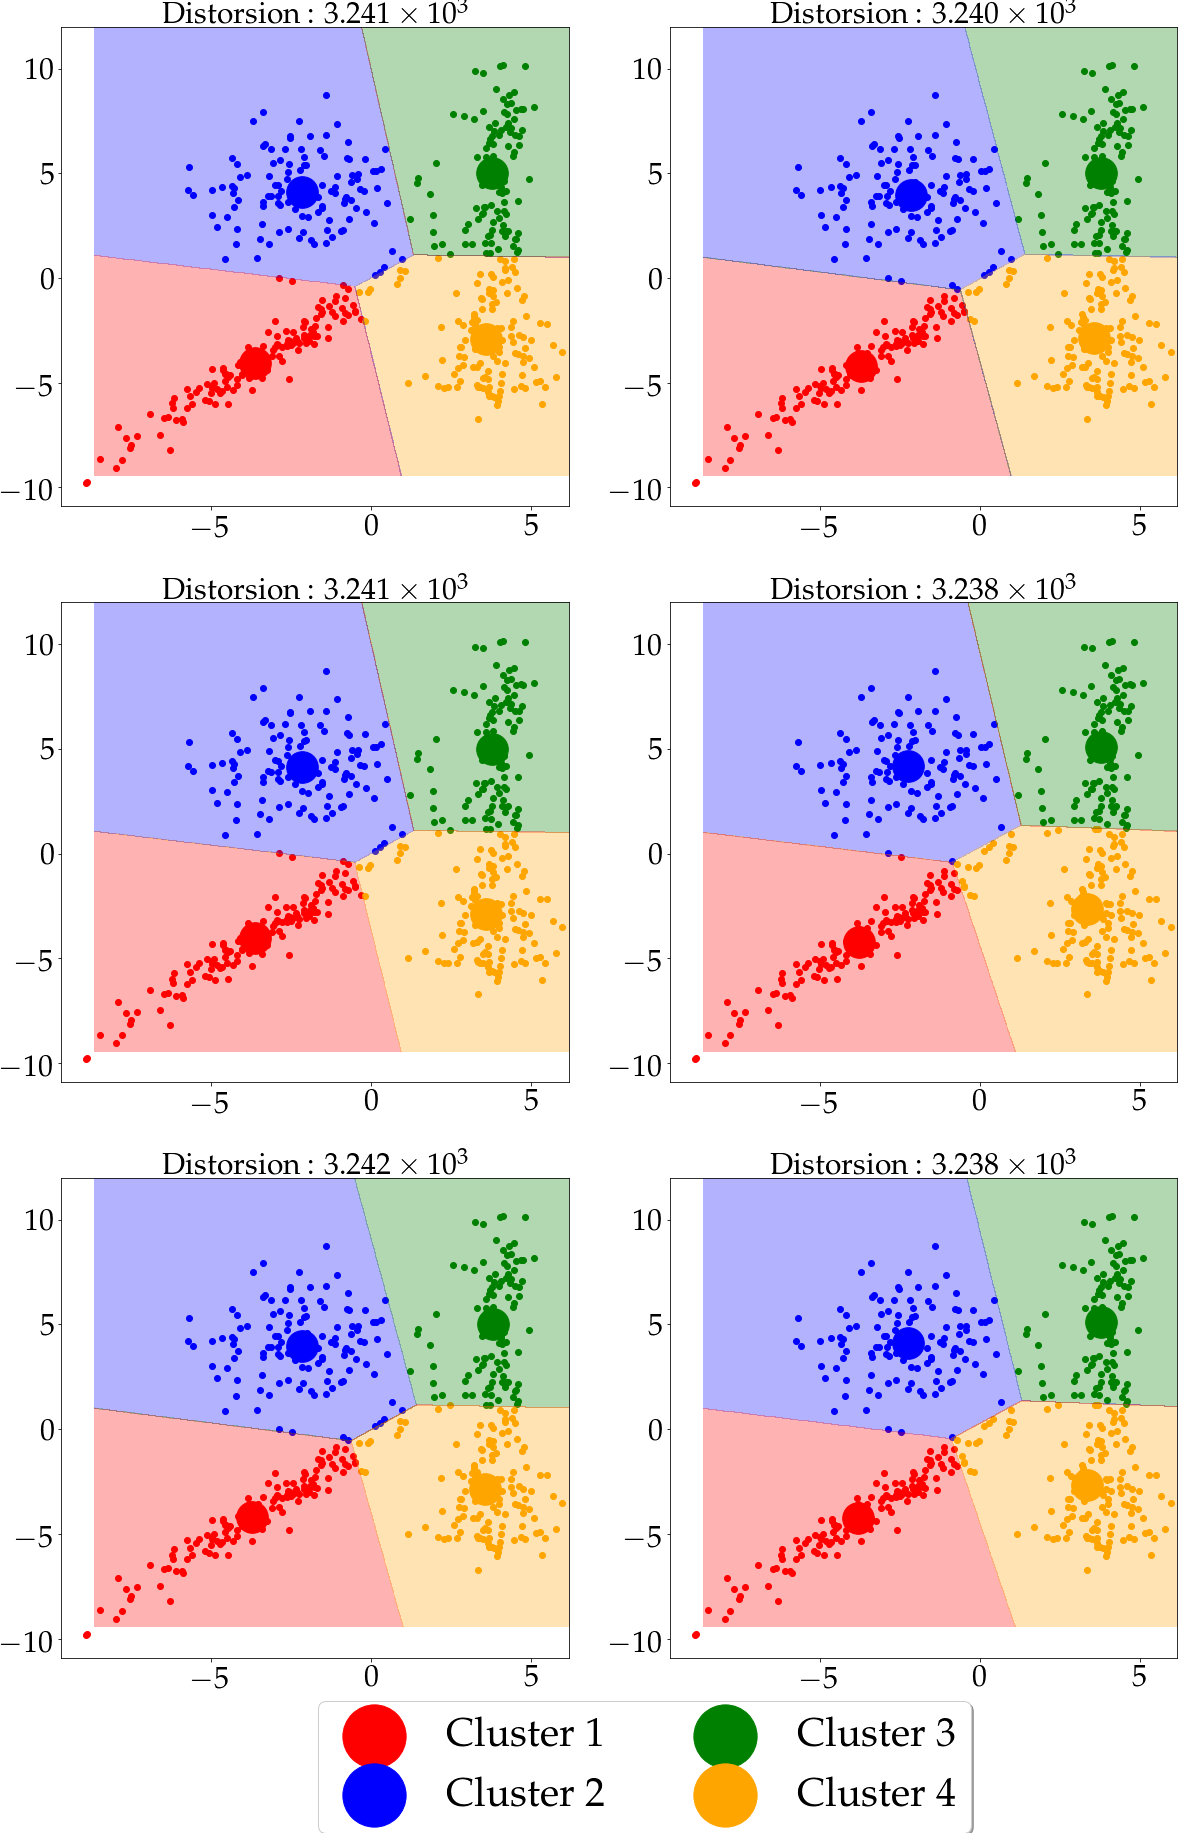
\includegraphics[width = \textwidth]{4_a}
	\caption{Visualisation du clustering obtenu par k-means des données d'entrainement sur 9 initialisations aléatoires des centroïdes}
	\label{fig_4_K_means}
\end{figure}

En figure~\ref{fig_4_K_means} sont présentés les résultats du clustering des données d'entraînement \textit{EMGaussian.data} avec 9 initialisations aléatoires distinctes des centroïdes. La condition d'arrêt est remplie quand la variation de distorsion est inférieure à 1. On a utilisé l'angle des centroïdes finaux afin d'artificiellement repérer par les mêmes couleurs et mêmes chiffres les clusters situés dans des zones similaires du plan. On constate que la distorsion de ces 9 initialisations différentes ne diffère que par le 3\up{e} chiffre significatif, avec une moyenne de \(3.239~10^{3}\) et avec un écart-type \(1.335\). Les minima locaux de cette distorsion ont donc des valeurs très semblables sur ces itérations, et les positions des centroïdes finaux sont regroupées dans la table~\ref{tab_4_a}. On peut constater que les variations autour des positions moyennes sont de l'ordre du dixième dans le pire des cas, correspondant à une variation en distance de l'ordre de \(0.3~\%\). Néanmoins on constate que les points à la frontière des clusters ont tendance à basculer, tantôt vers l'un ou l'autre des clusters, notamment à la frontière des clusters jaune bleu et rouge, où les points proches de \((0,0)\) sont facilement attribué par l'humain au cluster 1, rouge, qui présente une forme très allongée, différente des autres formes de clusters. Or la clusterisation par k-means ne permet pas de prendre en compte cette spécificité de forme. En définitif, les clusters trouvés par k-means sont, pour ce jeu de données d'entraînement, très stables pour la majorité des initialisations aléatoires et permette de séparer en première approximation, indépendamment de la forme du cluster, les points suivant un consensus proche de celui de l'homme, à l'exception de quelques points centraux.

\begin{table}
	\centering
	\begin{tabular}{r|r|r}
		\hline
		Centroïde & \(\mu_x \pm \sigma_x\) & \(\mu_y \pm \sigma_y\) \\\hline
		1         & \(-3.747\pm 0.068\)    & \(-4.193\pm 0.081\)    \\\hline
		2         & \( -2.177 \pm 0.044\)  & \( 4.060\pm 0.078 \)   \\\hline
		3         & \( 3.794\pm 0.007\)    & \( 5.038\pm 0.048\)    \\\hline
		4         & \( 3.483\pm 0.107\)    & \( -2.795\pm 0.105 \)  \\\hline
	\end{tabular}
	\caption{Positions des centroïdes sur les 9 initialisations aléatoires}
	\label{tab_4_a}
\end{table}

\subsection{Mixture de gaussiennes isotropiques}

Dans le cas d'une mixture de gaussiennes isotropiques, on peut réecrire l'étape de maximisation suivant :

\begin{equation}
	\begin{split}
		\bm{\theta}^{(t + 1)} &= \operatorname{arg}\max_{\bm{\theta}}\left(\mathbb{E}_{\bm{z} \mid \bm{x}, \bm{\theta}^{(t)}}\right)\\
		\bm{\theta}^{(t + 1)} &= \operatorname{arg}\max_{\bm{\theta}}\left(\sum_{n = 1}^N\sum_{k = 1}^4q_{nk}^{(t)}\left(\log\pi_k -
		\frac{1}{2}\log|\Sigma_k|-\frac{1}{2}\left(x_i - \mu_k\right)^{\intercal}\Sigma_k^{-1}\left(x_i - \mu_k\right)\right)\right)
	\end{split}
\end{equation}

où \(\bm{\theta} = \left(\bm{\pi}, \bm{\mu}, \bm{\Sigma}\right)\) et \(q_{nk}^{(t)} = \mathbb{P}\left(z_n = k | x_n, \bm{\theta}^{(t)}\right)\) avec \(z_n\) variable latente associée à \(x_n\).

On peut alors séparer la maximisation suivant \(\bm{\pi}\) et suivant \(\left(\bm{\mu}, \bm{\Sigma})\right)\), de sorte que :

\begin{equation}
	\begin{split}
		\bm{\pi}^{(t + 1)} &= \operatorname{arg}\max_{\bm{\pi}}\left(\sum_{n = 1}^N\sum_{k = 1}^4q_{nk}^{(t)}\log\pi_k\right) \quad \text{avec}\quad\forall n,\,\sum_{k = 1}^4q_{nk} = 1\\
		(\bm{\mu}^{(t + 1)}, \bm{\Sigma}^{(t + 1)}) &= \operatorname{arg}\max_{\bm{\mu}, \bm{\Sigma}}\left(\sum_{n = 1}^N\sum_{k = 1}^4q_{nk}\left(
		-\frac{1}{2}\log|\Sigma_k|-\frac{1}{2}\left(x_i - \mu_k\right)^{\intercal}\Sigma_k^{-1}\left(x_i - \mu_k\right)\right)\right)\\
	\end{split}
	\label{eq_isotrop}
\end{equation}

Les deux problèmes de minimisation en~\eqref{eq_isotrop} sont différentiables et concaves (le deuxième étant analogue au calcul du MLE pour une distribution normale) et on a :

\begin{equation}
	\begin{split}
		\frac{\partial\left(\sum_{n = 1}^N\sum_{k = 1}^4q_{nk}^{(t)}\log\pi_k^{(t+1)}\right)}{\partial\pi_k^{(t+1)}} &= \sum_{n = 1}^Nq_{nk}^{(t)} - \lambda \pi_k^{(t+1)} = 0 \quad \text{avec} \quad \lambda \in \mathbb{R}\\
		\pi_k^{(t+1)} &\propto \sum_{n = 1}^Nq_{nk}^{(t)}\\
		\pi_k^{(t+1)} &= \frac{\sum_{n = 1}^Nq_{nk}^{(t)}}{\sum_{k = 1}^4\sum_{n = 1}^Nq_{nk}^{(t)}} = \frac{1}{N}\sum_{n = 1}^Nq_{nk}^{(t)}
	\end{split}
\end{equation}


\begin{equation}
	\begin{split}
		\frac{\partial\left(\sum_{n = 1}^N\sum_{k = 1}^4q_{nk}^{(t)}\left(
		-\frac{1}{2}\left(x_i - \mu_k\right)^{\intercal}\Sigma_k^{-1}\left(x_i - \mu_k\right)\right)\right)}{\partial\mu_k} &=
		\sum_{n = 1}^Nq_{nk}^{(t)}\left(\Sigma_k^{-1}(x_i-\mu_k^{(t+1)})\right) = 0\\
		\mu_k^{(t + 1)} &= \frac{\sum_{n = 1}^Nq_{nk}^{(t)}x_i}{\sum_{n = 1}^Nq_{nk}^{(t)}}
	\end{split}
\end{equation}

Avec l'hypothèse \(\bm{\Sigma_k} = \sigma_k^2\bm{I}\) d'isotropie, il vient :


\begin{equation}
	\begin{split}
		\frac{\partial\left(\sum_{n = 1}^N\sum_{k = 1}^4q_{nk}^{(t)}\left(
		-\frac{1}{2}\log\sigma_k^4-\lVert x_i - \mu_k\rVert^2 / 2\sigma_k^2\right)\right)}{\partial\sigma_k^2} &=
		\sum_{n = 1}^Nq_{nk}\left(-\frac{1}{\sigma_k^2} +\frac{1}{2\sigma_k^4}\left(x_i-\mu_k\right)^{\intercal}\left(x_i-\mu_k\right)\right)\\
		&= 0 \\
		\sigma_k^2 &= \frac{\sum_{n = 1}^Nq_{nk}\left(x_i-\mu_k\right)^{\intercal}\left(x_i-\mu_k\right)}{2\sum_{n = 1}^Nq_{nk}}
	\end{split}
\end{equation}

En figure~\ref{fig_4_b} sont présentés les résultats de la mixture de gaussiennes isotropiques sur les mêmes données d'entraînement qu'en figure~\ref{tab_4_a}. La condition d'arrêt est atteinte quand la variation de la vraisemblance est inférieure à \(10^{-3}\). La même convention d'angle a été utilisé pour identifier les clusters délimités dans les zones semblables. La table regroupant les positions des centres est également présentée en table~\ref{tab_4_b}. On constate que la différence des positions des centres de masse par rapport à la position des centres de K-means est de l'ordre de grandeur de l'écart-type sur toutes les initialisations, de sorte qu'on peut conclure que la modélisation n'apporte pas de manière significative de changement dans les posistions des centres. En revanche, on constate que plusieurs extrema locaux de vraisemblance sont trouvés. En particulier, il peut arriver que tous les points proches de \((0,0\)) soit plutôt attribués au cluster 4 qu'au 3 autres (du moins, ces points peuvent avoir une variable lattente plus grande pour le cluster 4). On peut également observer des étalement de masse des gaussiennes différentes suivant les initialisations. Enfin, la vraisemblance moyenne pour cette mixture de gaussiennes isotropiques est de \((-2.642\pm0.003)~10^3\).

\begin{table}[b]
	\centering
	\begin{tabular}{r|r|r|r}
		\hline
		Centroïde & \(\mu_x \pm \sigma_x\) & \(\mu_y \pm \sigma_y\) & \(\lVert\Delta\mu\text{(kmeans-iso)}\rVert\) \\\hline
		1         & \(-3.991\pm 0.400\)    & \(-4.417\pm 0.411\)    & \(0.256\)                                    \\\hline
		2         & \( -2.441 \pm 0.166\)  & \( 4.278\pm 0.038 \)   & \(0.342\)                                    \\\hline
		3         & \( 3.252\pm 0.630\)    & \( 5.040\pm 1.437\)    & \(0.542\)                                    \\\hline
		4         & \( 3.229\pm 0.656\)    & \( -2.712\pm 1.101 \)  & \(0.267\)                                    \\\hline
	\end{tabular}
	\caption{Positions des centres de masse de chaque gaussienne représentée en figure~\ref{fig_4_b}, et norme de la différence des positions moyennes des centres pour k-means et des centres de masse des gaussiennes isotropiques.}
	\label{tab_4_b}
\end{table}

\begin{figure}[H]
	\centering
	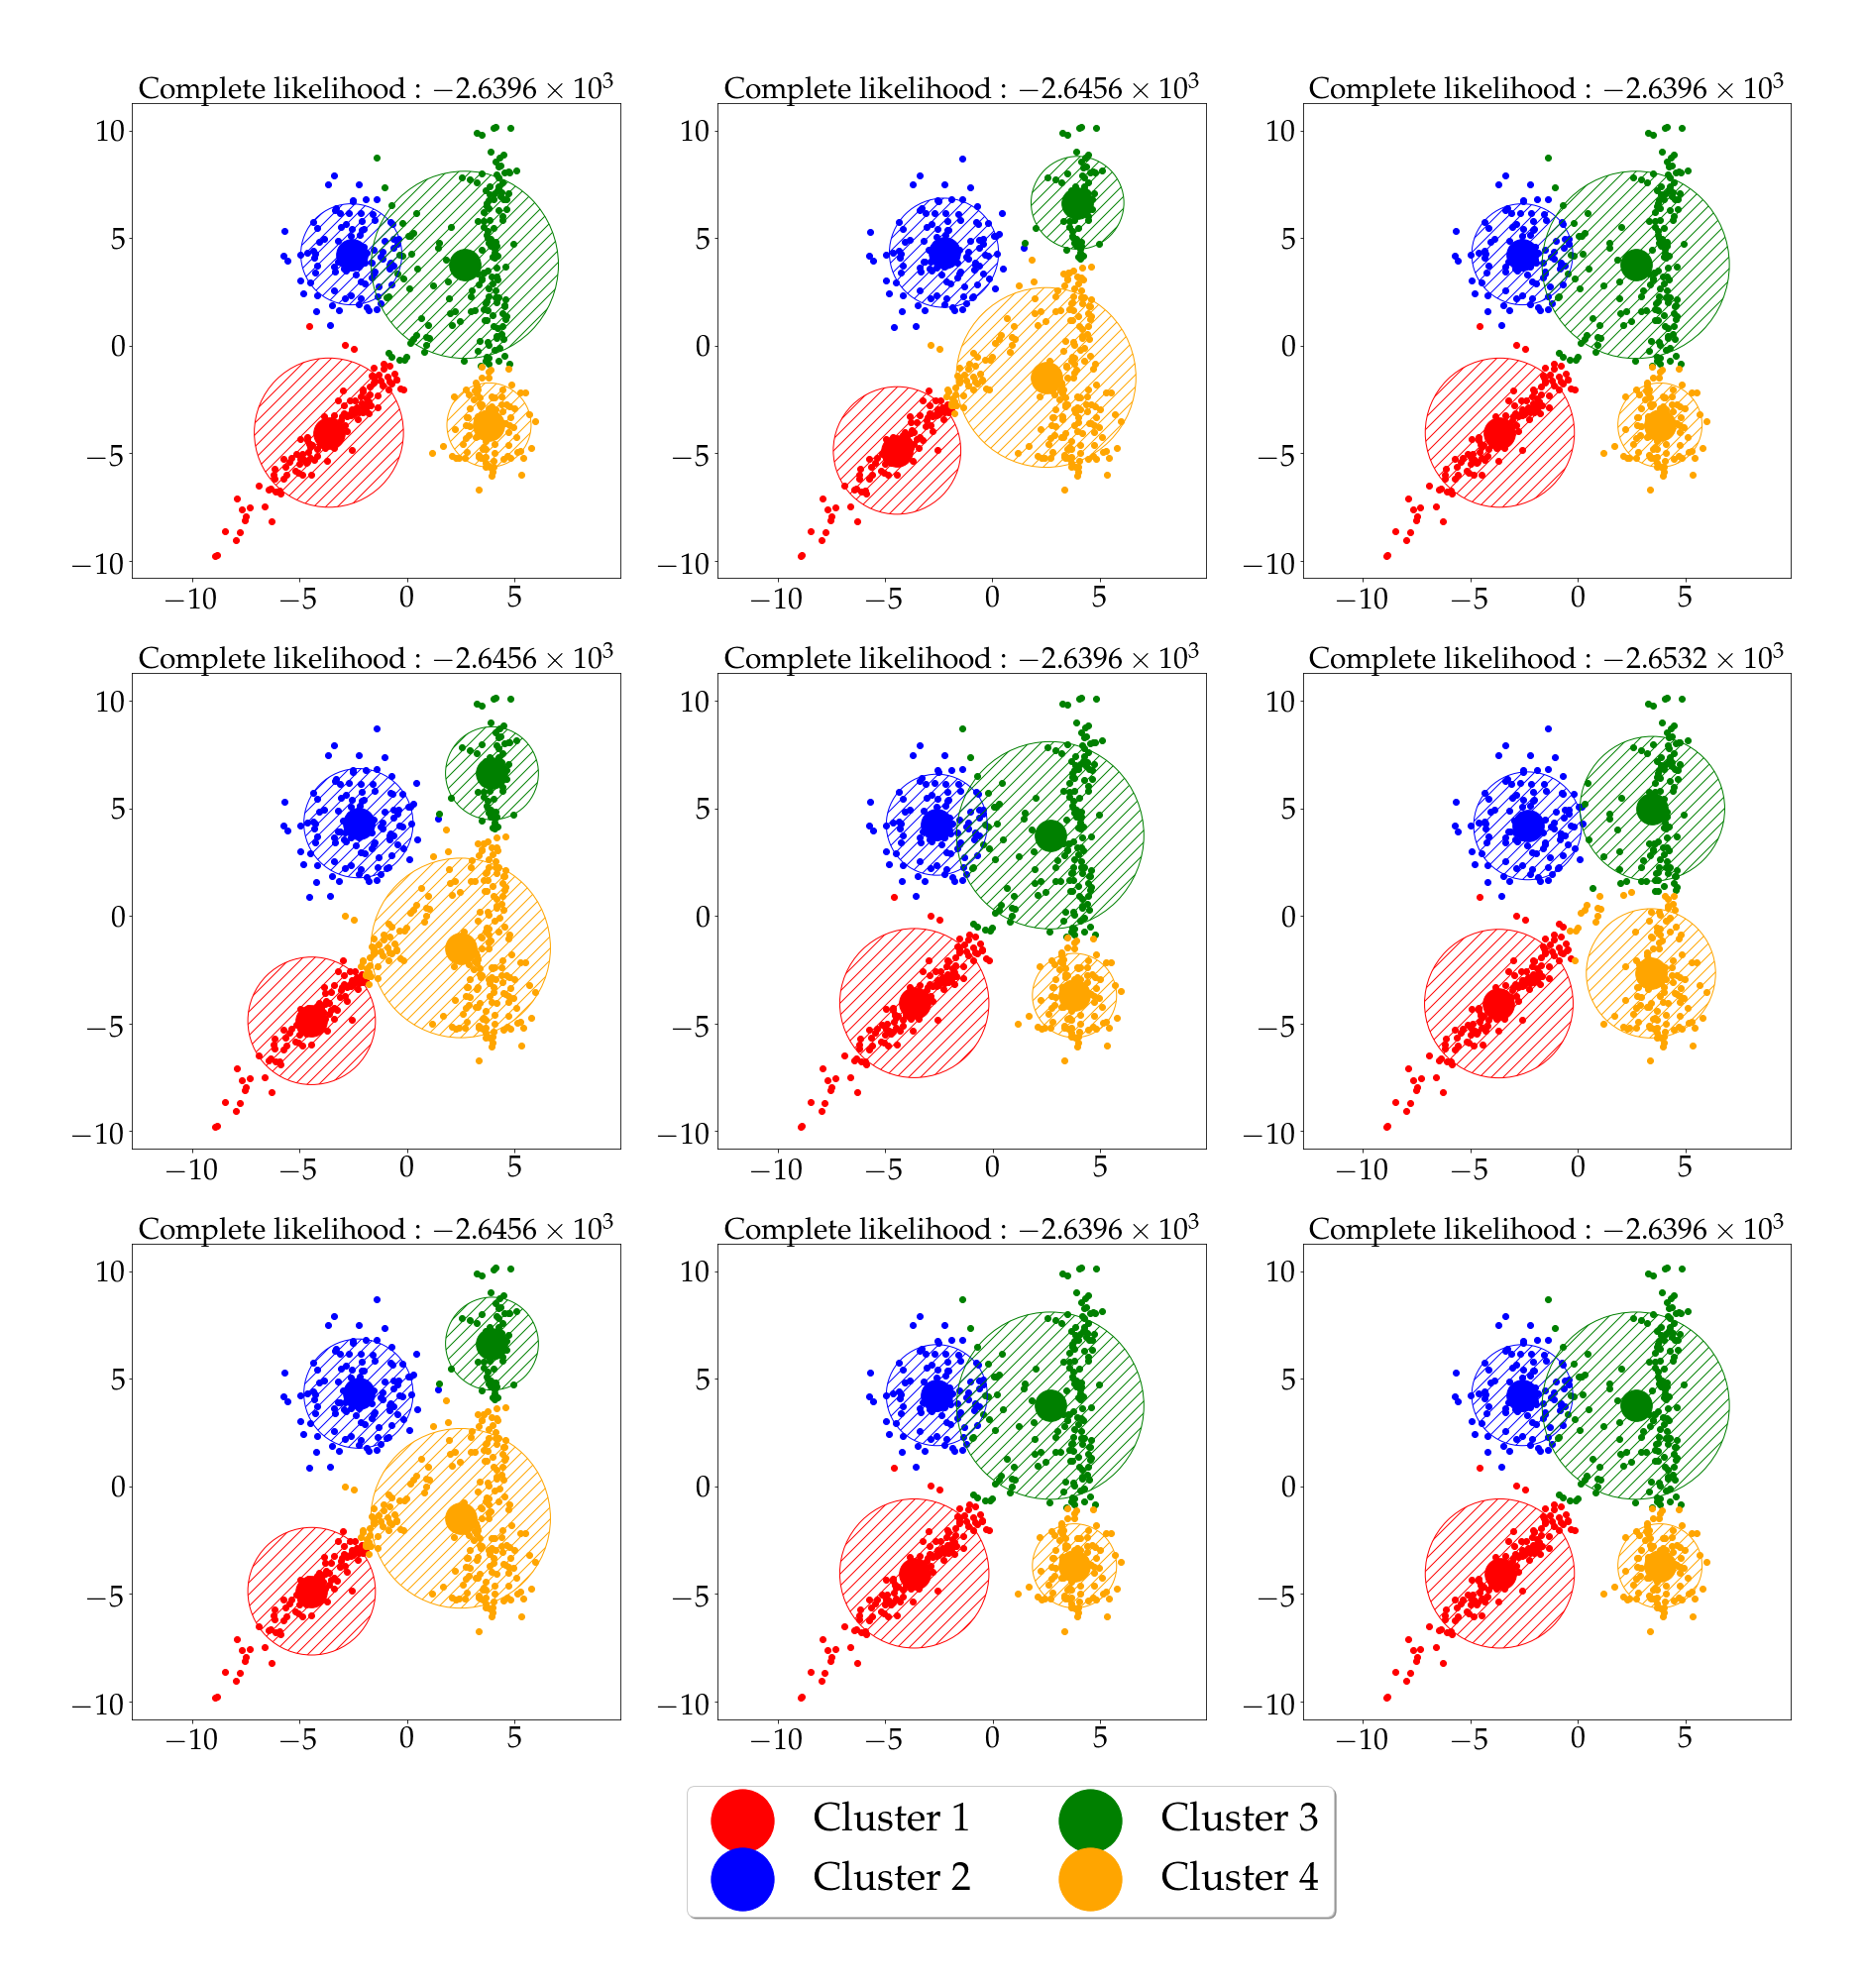
\includegraphics[width = \textwidth]{4_b}
	\caption{Visualisation du clustering obtenu par mixtures de gaussiennes avec des covariances isotropiques avec 9 initialisations par K-means des données d'entrainement. Chaque couleur représente un noeud gaussien. Le maxima des variables latentes de chaque point a été représenté, ainsi que la zone contenant \(90~\%\) de la masse de chaque gaussienne, en hachuré.}
	\label{fig_4_b}
\end{figure}


\subsection{Mixture de gaussiennes générales}

Sans l'hypothése d'isotropie, on a alors :

\begin{equation}
	\begin{split}
		\frac{\partial\left(\sum_{n = 1}^N\sum_{k = 1}^4q_{nk}^{(t)}\left(
		-\frac{1}{2}\log|\Sigma_k|-\frac{1}{2}\left(x_i - \mu_k\right)^{\intercal}\Sigma_k^{-1}\left(x_i - \mu_k\right)\right)\right)}{\partial\sigma_k^2} &= 0\\
		\Sigma_k = \frac{\sum_{n = 1}^Nq_{nk}\left(x_i-\mu_k\right)\left(x_i-\mu_k\right)^{\intercal}}{\sum_{n = 1}^Nq_{nk}}
	\end{split}
\end{equation}

En figure~\ref{fig_4_c} sont présentés les résultats de la mixture de gaussiennes avec covariance générale sur les mêmes données d'entraînement qu'en figure~\ref{tab_4_a}. La condition d'arrêt est atteinte quand la variation de la vraisemblance est inférieure à \(10^{-3}\). La même convention d'angle a été utilisé pour identifier les clusters délimités dans les zones semblables. La table regroupant les positions des centres est également présentée en table~\ref{tab_4_c}. On constate que les différences des positions des centres de masse entre le modèle isotropique et le modèle général sont largement supérieures, jusqu'à un facteur 4, comparées aux différences entre le passage du K-means à la mixture de gaussienne isotropique. La vraisemblance moyenne pour cette mixture de gaussiennes générales est de \((-2.327\pm0.000)~10^3\) et est inférieure à la vraisemblance obtenue pour la mixture de gaussiennes isotropiques. On constate, d'autre part, une très grande stabilité des positions des centres de masses, corroborée par la stabilité de la vraisemblance, pouvant mettre en évidence qu'un unique maximum a été atteint (qui n'est peut-être pas global). En l'occurence, sur ces données d'entraînement, les points en \((0,0\)) sont systématiquement attribués au cluster 1, du moins, en prenant le maximum des variables latentes comme attribution. Ce modèle permet de rendre compte des formes diverses des noeuds gaussiens, dont les distributions en masse sont tantôt allongés, tantôt regrouopées.

\begin{table}[b]
	\centering
	\begin{tabular}{r|r|r|r}
		\hline
		Centroïde & \(\mu_x \pm \sigma_x\) & \(\mu_y \pm \sigma_y\) & \(\lVert\Delta\mu\text{(iso-gen)}\rVert\) \\\hline
		1         & \(-3.060\pm 0.000\)    & \(-3.532\pm 0.000\)    & \(1.100\)                                 \\\hline
		2         & \( -2.034 \pm 0.000\)  & \( 4.173\pm 0.000 \)   & \(0.420\)                                 \\\hline
		3         & \( 3.981\pm 0.000\)    & \( 3.838\pm 0.005\)    & \(1.406\)                                 \\\hline
		4         & \( 3.800\pm 0.000\)    & \( -3.775\pm 0.000 \)  & \(1.207\)                                 \\\hline
	\end{tabular}
	\caption{Positions des centres de masse de chaque gaussienne représentée en figure~\ref{fig_4_c}, et norme de la différence des positions moyennes des centres de masses pour la mixture isotropique et générale.}
	\label{tab_4_c}
\end{table}


\begin{figure}[H]
	\centering
	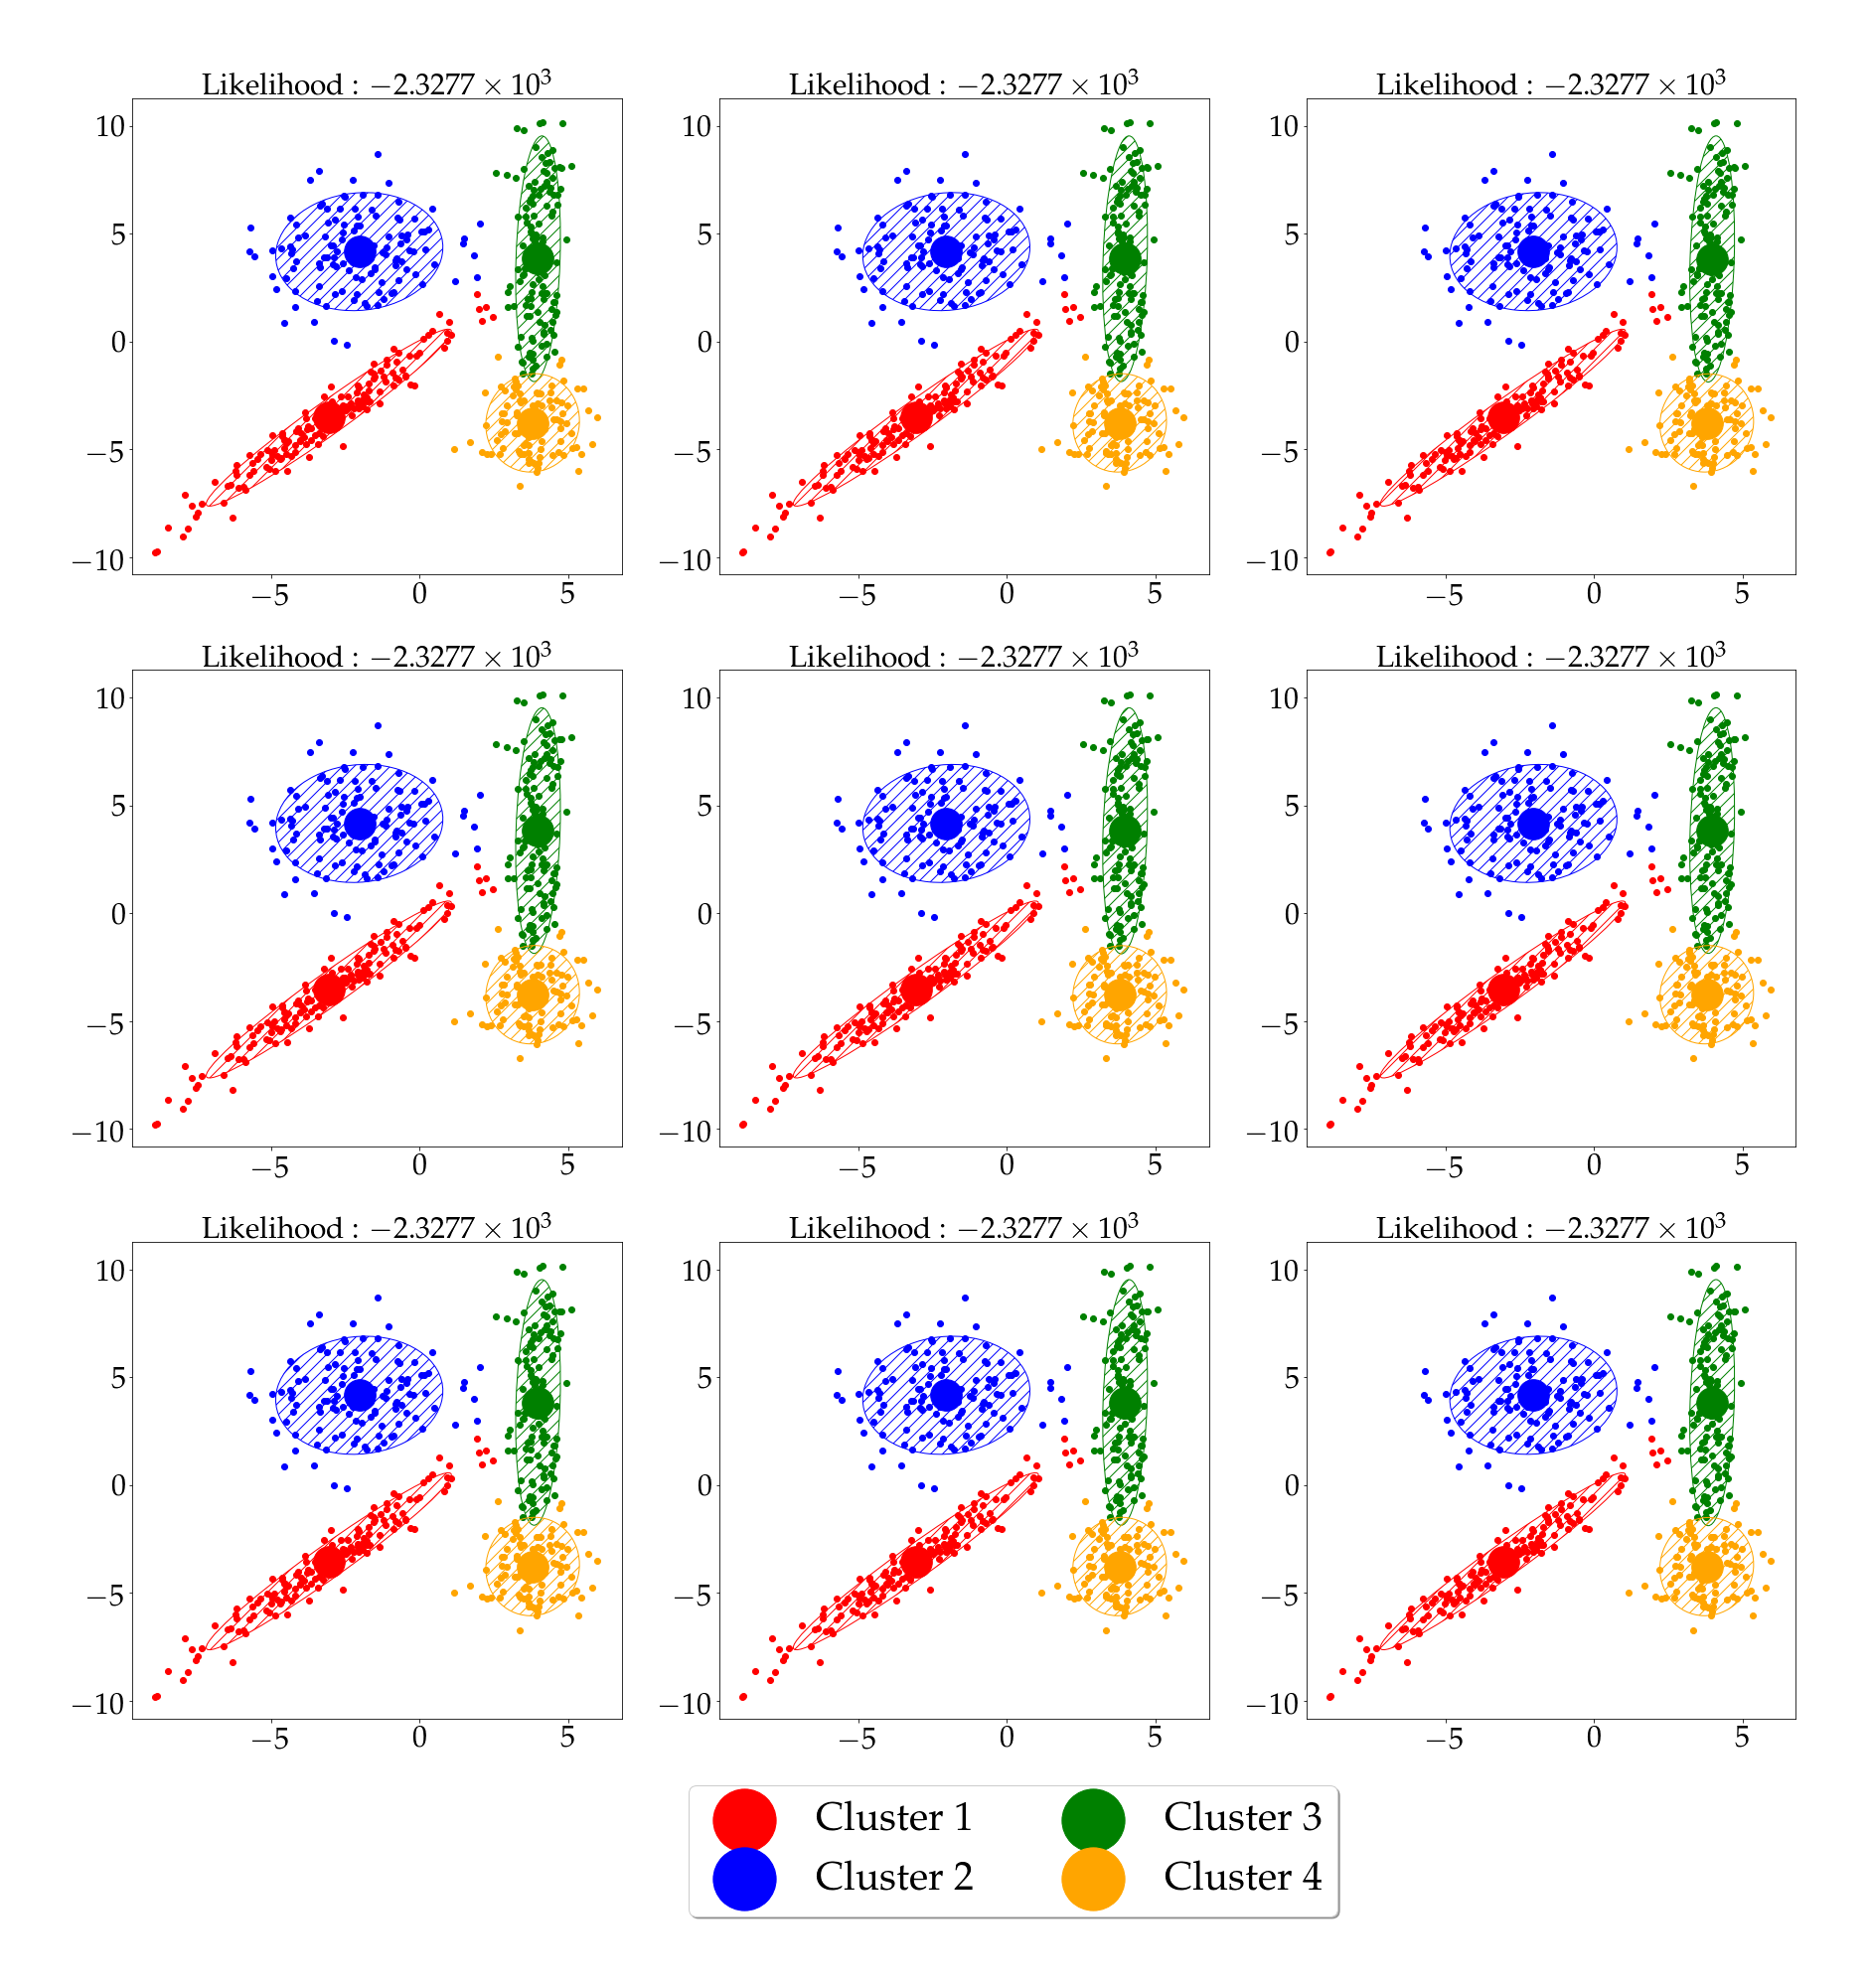
\includegraphics[width = \textwidth]{4_c}
	\caption{Visualisation du clustering obtenu par mixtures de gaussiennes avec covariance générale avec 9 initialisations par K-means des données d'entrainement. Chaque couleur représente un noeud gaussien. Le maxima des variables latentes de chaque point a été représenté, ainsi que la zone contenant \(90~\%\) de la masse de chaque gaussienne, en hachuré.}
	\label{fig_4_c}
\end{figure}

\subsection{Comparaison des résultats}

En figures~\refeq{fig_4_d_1},~\refeq{fig_4_d_2} sont présentés les résultats des deux mixtures de gaussiennes sur les données de test. On constate encore la grande stabilité en vraisemblance et en position des centre de masse, pour la mixture de gaussiennes générales, tandis qu'on observe toujours une instabilité en position et en forme des distribution pour la mixture de gaussiennes isotropiques. Pour cette dernière, la vraisemblance moyenne est de \((-2.593\pm0.037)~10^3\), inférieure à la vraisemblance de la mixture de gaussiennes générales, de \((-2.360\pm0.002)~10^3\), rendant bien compte de la modélisation plus adaptée du modèle général, avec des masses très allongées pour les clusters 1 et 3, qui ne sont pas bien rendues par des gaussiennes isotropiques.

\begin{figure}[H]
	\centering
	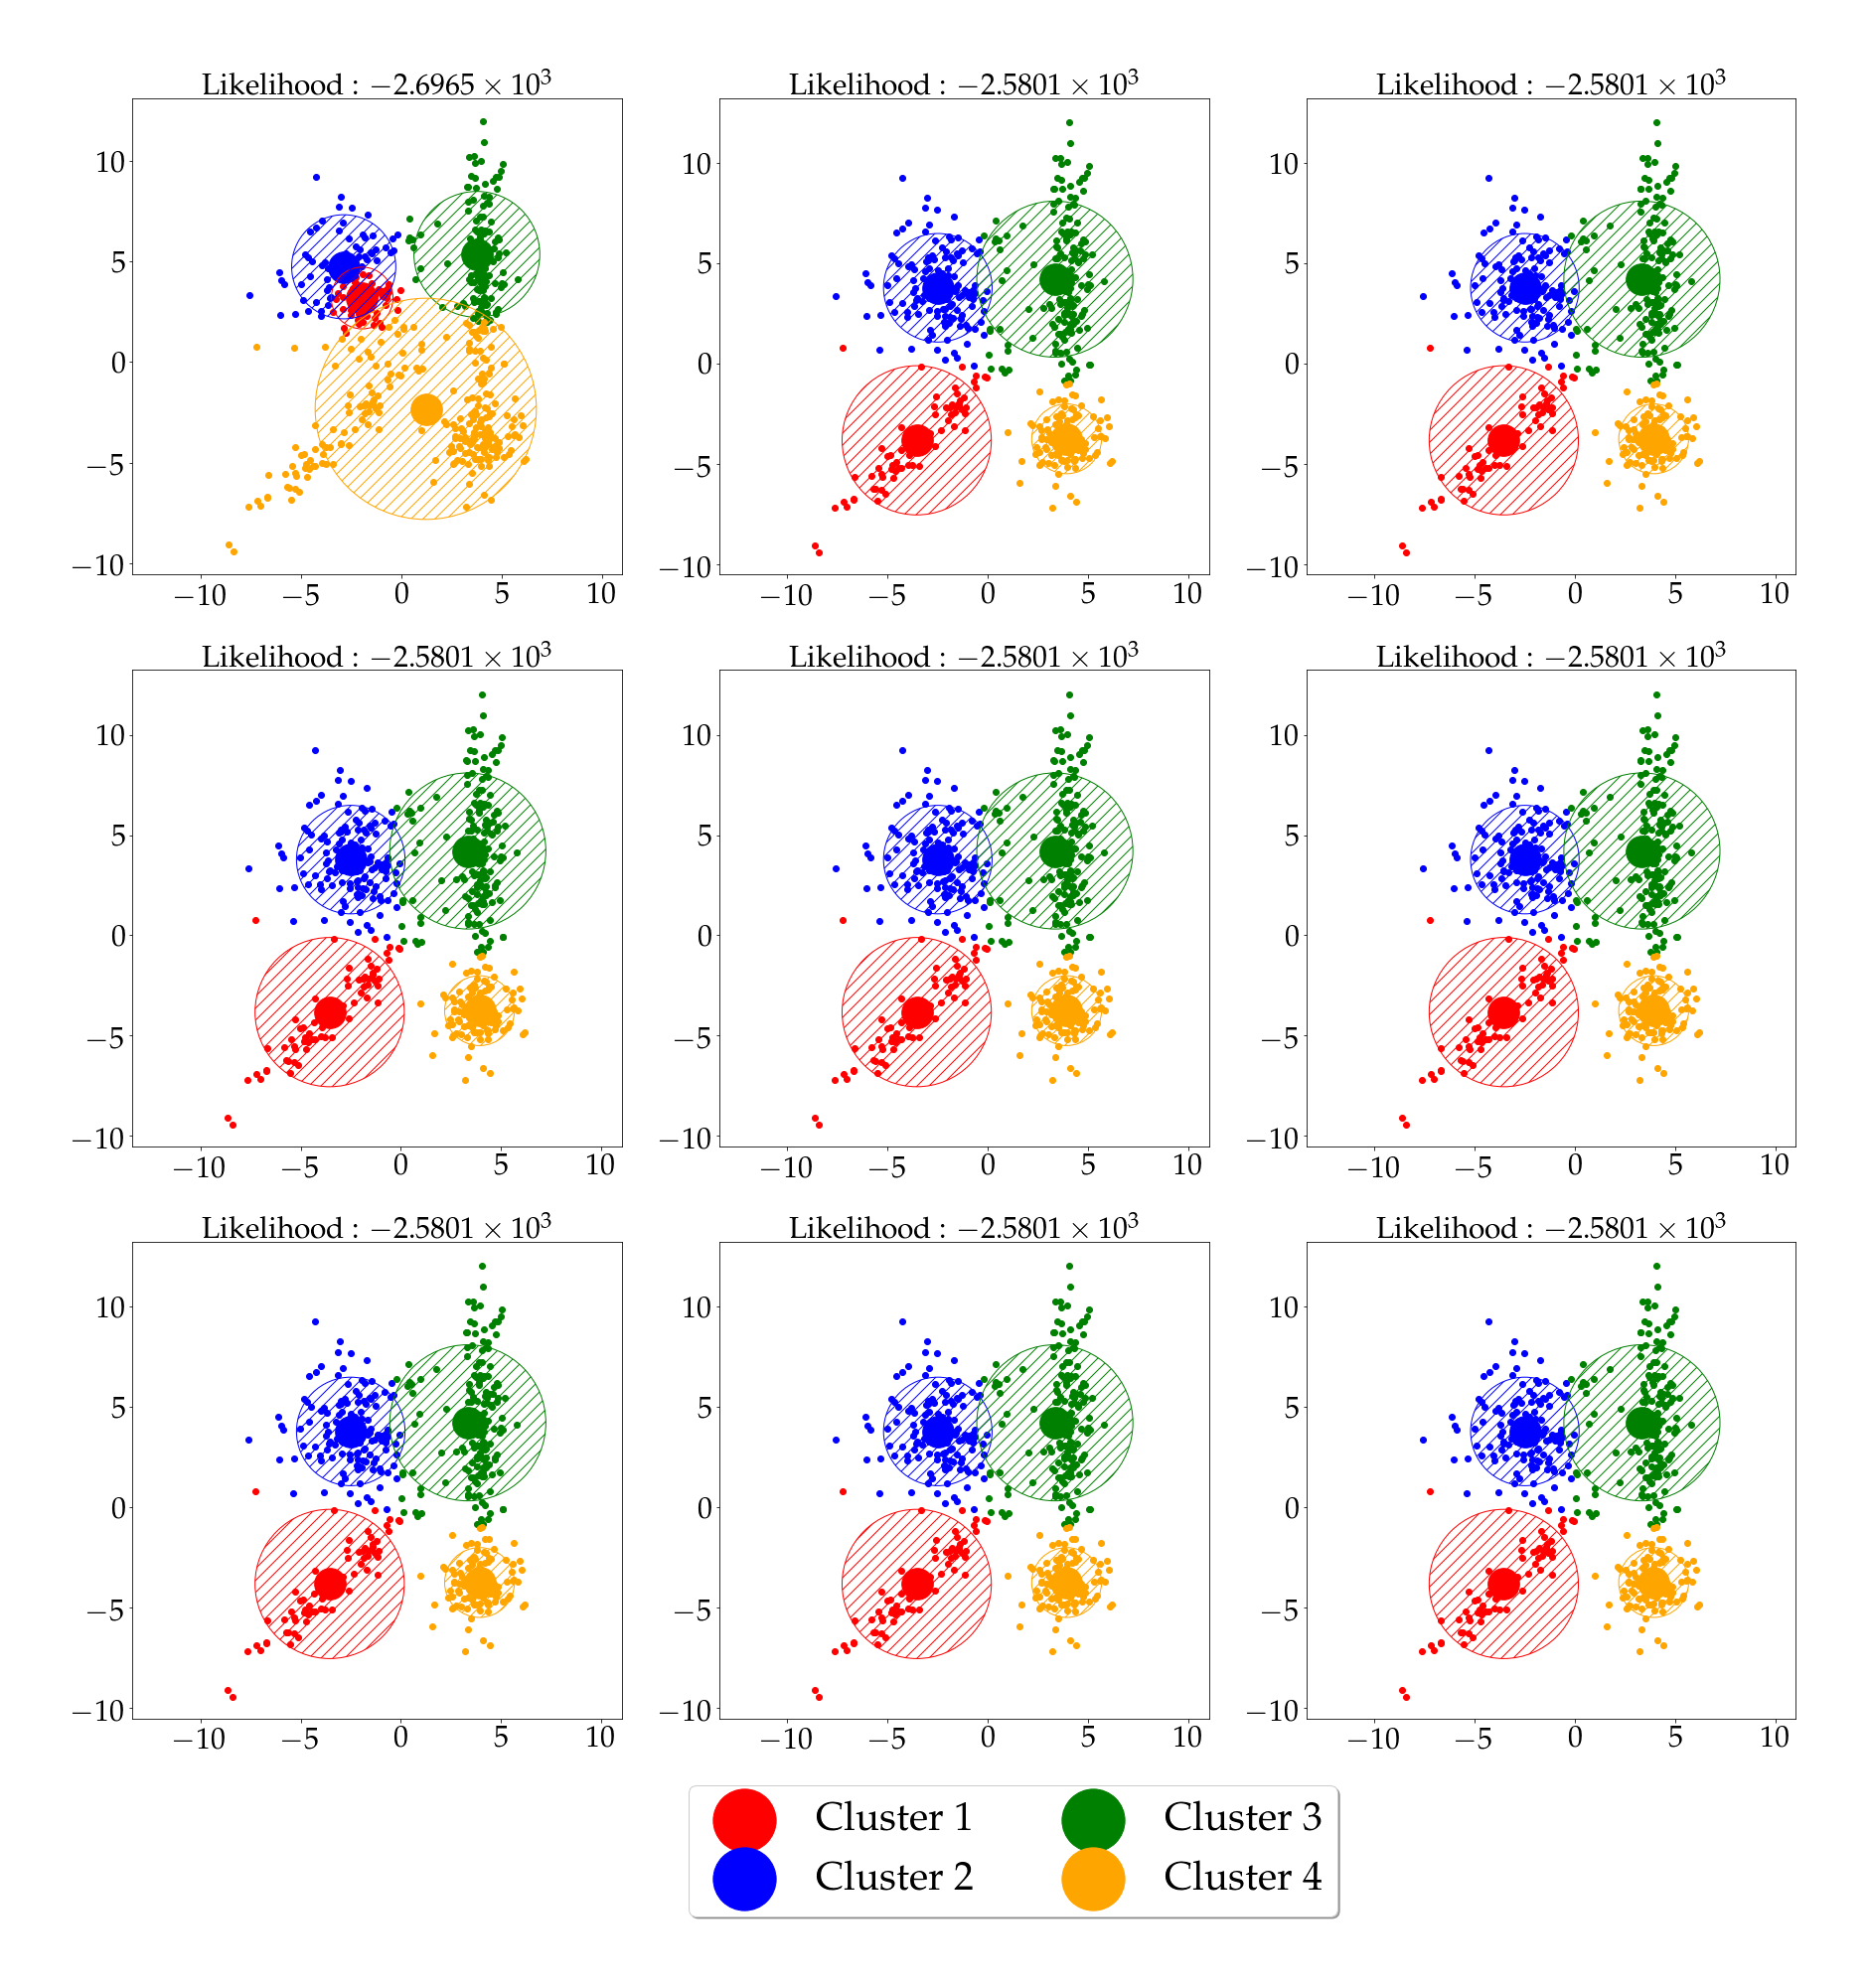
\includegraphics[width = \textwidth]{4_d_1}
	\caption{Visualisation du clustering obtenu par mixtures de gaussiennes avec des covariances isotropiques avec 9 initialisations par K-means des données de test. Chaque couleur représente un noeud gaussien. Le maxima des variables latentes de chaque point a été représenté, ainsi que la zone contenant \(90~\%\) de la masse de chaque gaussienne, en hachuré.}
	\label{fig_4_d_1}
\end{figure}


\begin{figure}[H]
	\centering
	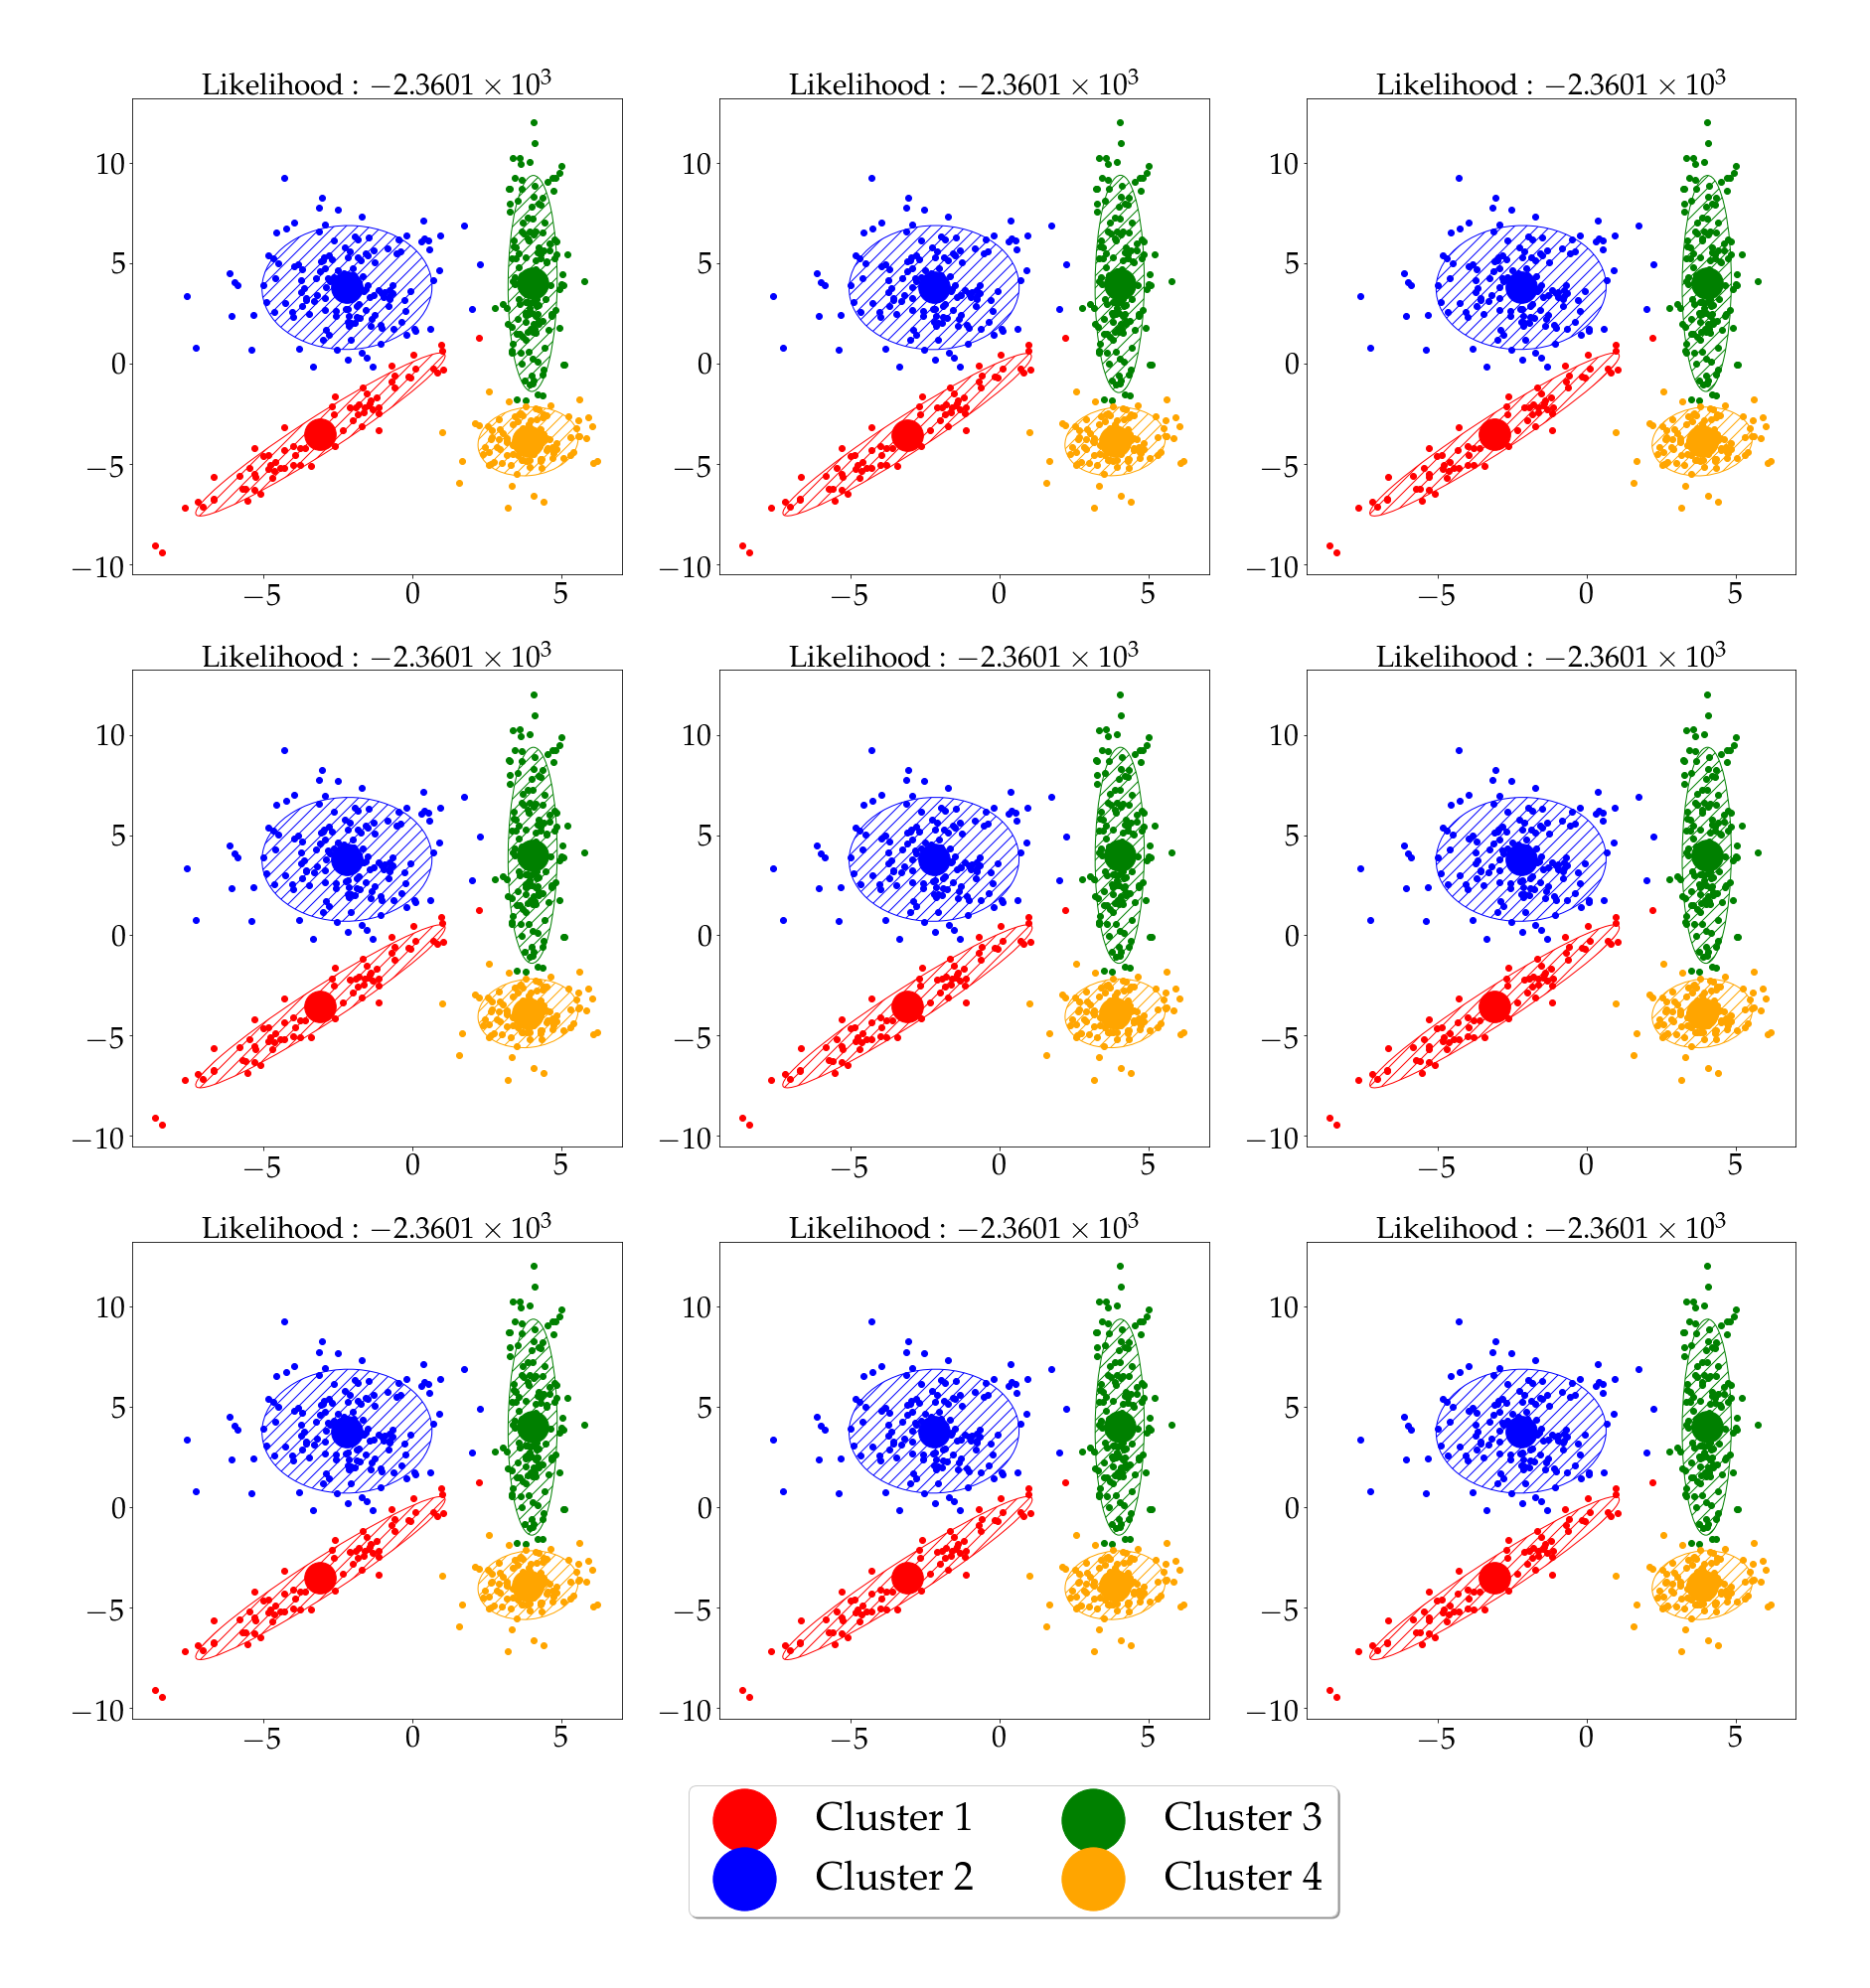
\includegraphics[width = \textwidth]{4_d_2}
	\caption{Visualisation du clustering obtenu par mixtures de gaussiennes avec covariance générale avec 9 initialisations par K-means des données de test. Chaque couleur représente un noeud gaussien. Le maxima des variables latentes de chaque point a été représenté, ainsi que la zone contenant \(90~\%\) de la masse de chaque gaussienne, en hachuré.}
	\label{fig_4_d_2}
\end{figure}

\end{document}
